\taskpic{ Через два блока, подвешенных на одной высоте, переброшена
  длинная нерастяжимая нить, к концам которой прикреплены два
  одинаковых груза. К середине нити прикрепляют ещё один такой же
  груз и отпускают без начальной скорости. Расстояние между осями
  блоков равно $2l$. Чему равно ускорение центрального груза когда он
  проходит положение равновесия? }
{
  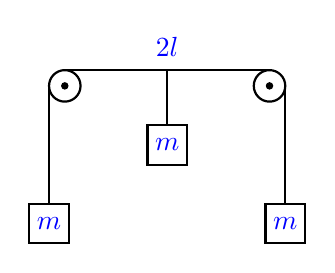
\begin{tikzpicture}
    \draw[thick] (0.7,2) circle (0.2) (3.3,2) circle (0.2);
    \draw[thick] (0.5,2) -- (0.5,0) (3.5,2) -- (3.5,0);
    \draw[thick] (0.7,2.2) -- (3.3,2.2);
    \draw[thick,fill=white] (0.25,0.5) rectangle (0.75,0) node[blue,midway]
    {$m$};
    \draw[thick,fill=white] (3.25,0.5) rectangle (3.75,0)
    node[blue,midway] {$m$};
    \draw[thick] (2,2.2) -- (2,1.5);
    \draw[thick,fill=white] (1.75,1.5) rectangle (2.25,1)
    node[blue,midway] {$m$};
    \draw[fill=black] (0.7,2) circle (0.04) (3.3,2) circle (0.04);
    \draw (2,2.5) node[blue] {$2l$};
  \end{tikzpicture}
}
% Слободянюк, "Очень длинные физические задачи"
